%\documentclass[twocolumn,superscriptaddress,showpacs,preprintnumbers,amsmath,amssymb,prl]{revtex4-1}
\documentclass[twocolumn,showpacs,amsmath,amssymb,pre,superscriptaddress]{revtex4}
\usepackage[utf8]{inputenc}
\usepackage{graphicx}% Include figure files
\usepackage{amsmath}
\usepackage{amssymb}
\usepackage{color}
\usepackage{comment}
\usepackage{siunitx}
%\usepackage{dcolumn}% Align table columns on decimal point
%\usepackage{bm}% bold math

%\graphicspath{{./FIGS/}}

\begin{document}

%\title{``Colloidal rain'', an alternative route to gelation during viscoelastic phase separation}
%\title{Colloidal rain: a novel crystallization pathway following viscoelastic phase separation}
\title{Novel crystallization pathway\\and formation of ``colloidal rain'' during viscoelastic phase separation}
\author{Hideyo Tsurusawa}
\affiliation{Institute of Industrial Science, University of Tokyo, 4-6-1 Komaba, Meguro-ku, Tokyo 153-8505, Japan}
\author{John Russo}
%\email{russoj@iis.u-tokyo.ac.jp}
\affiliation{Institute of Industrial Science, University of Tokyo, 4-6-1 Komaba, Meguro-ku, Tokyo 153-8505, Japan}
\author{Mathieu Leocmach}
\affiliation{Institut Lumière Matière, CNRS UMR 5306, Université Claude Bernard Lyon 1, Université de Lyon, Lyon, 69622 Villeurbanne Cedex, France}
\author{Hajime Tanaka}
%\email{tanaka@iis.u-tokyo.ac.jp}
\affiliation{Institute of Industrial Science, University of Tokyo, 4-6-1 Komaba, Meguro-ku, Tokyo 153-8505, Japan}


\date{\today}

\begin{abstract}
{
Colloidal gels form when network-forming spinodal phase separation is interrupted by the glass transition~\cite{lu2008gelation}. It has been shown that crystallization may equivalently interrupt the phase separation by freezing the dense phase. However the particle-level details of this process have not yet been confirmed experimentally.
Here we show by confocal microscopy measurements that crystallisation leads to a network structure different from the original phase separation pattern. Crystals nucleate inside the liquid network, and grow past it by direct condensation of the gas phase on their surface, driving evaporation of nearby liquid.
This process represents the colloidal analogue of the Bergeron process~\cite{glickman2000glossary}, i.e. ice crystals formation that occurs in mixed phase clouds and is at the origin of rain. Our \emph{colloidal rain} gives us full experimental access to the kinetic pathway of this phenomenon important for climate science.
We argue that states similar to colloidal rain can form as the result of the gas-liquid phase separation of crystallizable components, such as monoatomic and molecular systems, whose dynamics is slow enough to induce viscoelastic phase separation, but fast enough to prevent immediate vitrification.
}
\end{abstract}
 
\maketitle
Gels and glasses are two important non-ergodic disordered states, which are very important 
in our life and nature~\cite{anderson2002insights,lekkerkerker2011colloids}.
The dynamical arrest of colloidal gels and glasses is believed to originate from a dynamical transition to the same non-ergodic disordered glass state, i.e., vitrification. The only difference comes from the fact that the former is formed by densification induced by phase separation and thus is spatially heterogeneous, whereas the latter is formed by uniform densification and is thus spatially homogeneous.
Gels are distinct from glasses because of their heterogeneous network structure, which gives them properties intermediate between
those of a solid and a fluid phase, and allows the coexistence of two properties usually incompatible with each other, 
elasticity and fluid transport. 
The elasticity of gels originates from the percolated network structure and the resulting space-spanning connectivity. 
At the same time a fluid component can easily flow through the elastic network.
There are two types of gels with such characteristics: one is a network structure stabilized by stable crosslinks, and the other is a phase-separated structure frozen by dynamical arrest due to vitrification.
Many chemical and physical gels belong to the former category, in which the size of network pores is rather small and 
the fluid transport is not so efficient. On the other hand, gels made of spherical colloids and proteins 
with attractive interactions belong to the latter category. 
This type of gels are formed by viscoelastic phase separation \cite{tanaka1999colloid,tanaka2000viscoelastic} into a dense liquid phase with slow dynamics and a dilute gas phase 
with fast dynamics. This difference in the viscoelastic properties between the two phases allows the system to form a space-spanning 
network structure of the liquid phase, even if it is the minority phase. During phase separation, the density of the liquid phase 
increases towards the glass-transition density, leading to slow glassy dynamics.
At the glass transition point, the percolated network structure is dynamically stabilised by vitrification 
of the dense liquid phase~\cite{pusey1993dynamics,ilett1995phase,verhaegh1997transient,tanaka1999colloid,foffi2002,zaccarelli2007,lu2008gelation,zaccarelli2008gelation,testard2011}.  
More precisely, the dynamical stabilization is due to percolation of locally favoured structures, which are locally stable non-crystalline structures \cite{royall2008g}.
% Since ``glass'' is the term used for bulk, this may be a more appropriate way to express the mechanism of dynamical arrest. 
% This type of gels are made by phase separation. Thus, the structure is intrinsically heterogeneous, and the network pore size is usually 
% much larger than gels made of stable crosslinks, resulting in a high fluid transport ability. 

Unlike the above standard scenario of colloidal gelation, it is known that phase separation can also be arrested by crystallization, if the process takes place below the melting point of a component of a mixture~\cite{tanaka1985new}. 
Indeed the possibility of a different class of gels, which are stabilised by crystallization, 
was suggested by numerical simulations~\cite{fortini2008crystallization,perez2011pathways} and observed in microgravity experiments \cite{sabin2012}.
For colloidal systems, we can in principle access structural evolution in real time at a single-particle level; however, there has so far been no confocal microscopy  
study on the process of crystal-gel formation. The main difficulty consists in the preparation protocol, where a colloidal-polymer mixture undergoes
shaking or shear before observation of its dynamics. This introduces turbolent flows at the beginning of the process, and also does not allow the
observation of the first stages of crystallization.
In our experiments we instead succeed in building a novel setup that allows the time evolution of the system to be observed directly
under the confocal microscope from the very early stages and without introducing fluid flows.

Our results show that, for low polymer concentration, the system can undergo a novel crystallization pathway that leads to the formation
of crystalline droplets. These droplets originate from crystal seeds that form inside the liquid branches of the spinodal aggregate, but then grow by direct condensation from the gas phase. The process is analogous to the Bergeron process of ice formation in mixed phase clouds, where ice droplets grow at the
expense of the supercooled liquid droplets due to their lower saturated vapour pressure. In our colloidal system, we then call this process ``colloidal rain''
formation. Due to the difference in the nucleation and growth processes, the droplets display different scaling laws depending on their
size. For small nuclei, the droplets have the same fractal dimension of the embedding gel network. But during the growth process, droplets
grow with an integer fractal dimension due to direct condensation of gas particles. This is in contrast to the standard crystal-gel scenario, where crystals nucleate and grow inside the dense branches of the gel, becoming dynamically arrested. We also observe that increasing the strength of the interparticle attraction
(by increasing the polymer concentration), instead of forming colloidal rain, the system undergoes the classical gelation process, in which
phase separation is interrupted by vitrification~\cite{lu2008gelation}.


\subsection*{Experiments}

In our experimental setup, the sample cell is put in contact with a reservoir of a salt solution through a semi-permeable membrane.
At $t=0$, the increase in the concentration of salt ions progressively screens the Coulombic repulsion between colloidal particles,
which are then subject to attractive depletion forces, making the system thermodynamically unstable and leading to phase separation (see Methods).
%In the following we discuss all the stages of the formation of the crystal gels: phase separation, stress-driven agein and crystallization.
The experimental data is taken at two different volume fractions ($\phi=0.10$ and $\phi=0.25$) and for different values
of the polymer concentration, $c_p=0.38,0.48,0.57,1.07$ for $\phi=0.25$ and $c_p=0.82,1.36$ for $\phi=0.10$.
In Fig.XXX we superimpose the state points with the phase diagram calculated from the YYY equation of state.
For each state points, scans at early times (every $10s$) and at the late stage (every $30s$) of the gelation process.
{\color{blue}We need more details of the experiments here}.

%
%\subsection*{Phase separation}
%
%In Fig.~\ref{fig:gel}a we show the cluster size distribution for all state points at their gelation point. The decay of the distribution
%follows different power laws $n(s)\sim s^\tau$, where $\tau$ is the Fisher exponent \cite{family2012kinetics}.
%For state points with $\phi=0.25$ the decay is well described by the three dimensional (3D) random percolation exponent $\tau=2.18$ \cite{family2012kinetics}.
%For state points with $\phi=0.10$, on the other hand, the decay appears to be slower, close to the diffusion limited cluster aggregation (DLCA) 
%exponent $\tau=1.8$ \cite{family2012kinetics}. While it is plausible that gelation at lower volume fraction occurs through cluster aggregation, especially given 
%the high polymer concentration of these state points, we have to warn that the cluster size distribution is very sensitive to
%experimental conditions and statistical noise (which is high in our case since the distributions are extracted from a single frame).
%Other measures of fractal dimensions (see below) will in fact suggest that also the $\phi=0.10$ states belong to the random gel universality class.
%
%Next we show in Fig.~\ref{fig:gel}b the radius of gyration $R_{\rm g}$ for the clusters of size $s$ at the gel point. All clusters, irrespective
% of the state point, follow the power-law: $R_{\rm g}\sim s^{2/D}$, with $D=2.53$ the fractal dimension in the random gelation
% universality class \cite{family2012kinetics}. So far, we have thus proven that, in the initial stages of phase separation, the liquid branch is
% formed by colloidal particles that aggregate to form a random gel.
% 
% Even after a gel is formed, the system keeps evolving.
% However, since a gel has an elasticity due to its space-spanning connectivity, the process should be markedly different from 
% ordinary fluid phase separation. Now we consider this unique feature of the coarsening of a gel network.  
% 
% \subsection*{Stress-driven ageing}
% 
% Previous simulation results~\cite{tanaka2000,tanaka2007spontaneous,furukawa2010key} have suggested that hydrodynamic interactions play
% a key role in the process of colloidal gelation. Without hydrodynamic interactions, particles have the tendency to
% aggregate in compact structures and subsequently form thick network structures. This also limits the possibility to
% form arrested gel states only at relatively high volume fractions. With hydrodynamic interactions, particles first form
% a transient gel even at very low volume fractions, and only later they increase the number of
% nearest neighbours to minimize the energy of the structure. 
% Thus, hydrodynamic interactions lead to the formation of gels that are very far from equilibrium and under a strong thermodynamic driving force 
% towards more stable compact structures. 
% The resulting transition from open to more compact networks occurs only through
% the breaking of the bonds that have accumulated more stress. The process was called stress-driven ageing~\cite{tanaka2007spontaneous}, 
% which is characteristic of viscoelastic phase separation \cite{tanaka2000viscoelastic}. 
% Below we provide the first experimental proof of this process.
% 
% In Fig.~\ref{fig:stress}a, we plot the fraction of liquid and gas particles as a function of time during phase separation
% at the state points of $\phi=0.10$. We observe that at high polymer concentration ($c_p=1.36$, dashed lines) both the
% liquid and gas branch change monotonically with time as the phase separation proceeds. At low polymer concentration
% ($c_p=0.82$, continuous lines), on the other hand, we find a non-monotonic evolution of both the liquid and gas branches, which is signalling
% a structural reorganization of the network. To prove that this is indeed a stress-driven ageing process, in Fig.~\ref{fig:stress}b 
% we plot the average number of bond-breaking events for the low-polymer concentration state point. The figure clearly shows that
% the network restructuring follows a peak in the number of bond-breaking events. We have thus found direct evidence of the
% stress-driven ageing process in colloidal gels that is a direct consequence of the formation of a thin network with the help of hydrodynamic interactions in the first stages
% of the aggregation process.
% 
% In Fig.~\ref{fig:stress}c we plot the time evolution of the structure factor, $S(q)$, for the state point
% undergoing network reorganization $\phi=0.10$ and $c_p=0.82$. The time of network reorganization as found in Fig.~\ref{fig:stress}a and b
% corresponds to a steep increase of the low wavenumber scattering from the network, that signals the coarsening of the network structure. 
% 
% The same conclusions also hold for the state point at $\phi=0.25$. We observe network restructuring only for the state point
% at lower polymer concentration, $c_p=0.38$. Interestingly, this is also the only state point that undergoes crystallization,
% meaning that the coarsening of the network of the dense liquid phase and the resulting formation of a wider liquid branch is a necessary condition for crystallization. 

\subsection*{Results}


\begin{figure*}[!t]
 \centering
 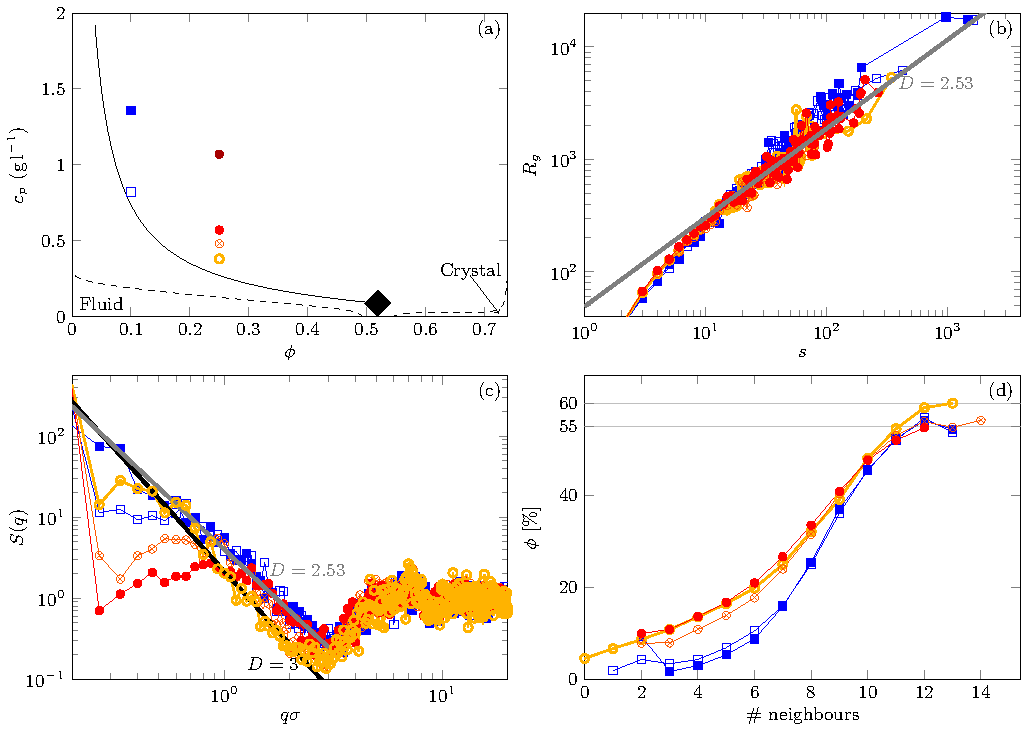
\includegraphics{./fig/phase_separation.pdf}
 \caption{{\bf Different routes of viscoelastic phase separation.}
 \textbf{a,} Phase diagram. Dashed lines are fluid-solid equilibrium coexistence boundaries. The continuous line is the gas side of the metastable gas-liquid spinodal region with the black diamond marking the critical point. The other symbols are the experimental points, consistently used in all panels.
 \textbf{b,} Radius of gyration ($R_g$) as a function of cluster size ($s$) for all state points at percolation. The
 gray line represents the fractal dimension of the random gelation universality class.
 \textbf{c,} Structure factors for the late stages of the gelation process. The gray and black lines represents respectively random gelation and compact fractal dimensions.
 \textbf{d,} Local volume fraction around a colloidal particle, as a function of the number of nearest neighbours of the particle \textcolor{blue}{at late stage?}. Horizontal lines stress the value at 12 neighbours.
 }
 \label{fig:phase_separation}
\end{figure*}

All samples share the same early time stages of spinodal decomposition. First the colloidal particles start aggregating,
eventually forming a percolating network. Then liquid-gas phase separation takes place, in which a dense network (liquid)
coexists with freely diffusing monomers (gas). The topology of the network is similar to all our samples at the initial stages.
This is shown for example in Fig.~\ref{fig:phase_separation}b, where we plot the radius of gyration of colloidal clusters ($R_g$)
as a function of the cluster size ($s$) at the percolation point. Two particles belong to the same cluster if their distance is
within the first peak of the radial distribution function. All samples show the same scaling law, which is compatible with
the random gelation universality class exponent ($D=2.53$) as shown by the dashed line in Fig.~\ref{fig:phase_separation}b.

While sharing similar structural properties at early times, the samples differ during the later stages of the phase separation process.
To examin this in more detail, we plot in Fig.~\ref{fig:phase_separation}c the structure factor for the final stages of the gelation process for all state points.
Calculation of the structure factor is done with the Hanning window function, to minimize boundary effects.
The figure shows that at low wavenumber $q$, the structure factor displays fractal scaling compatible with Guinier law, $S(q)\sim q^{-D}$.
But a difference
in the fractal dimension $D$ between the $\phi=0.25$ and $c_p=0.38$ state point and other state points starts to become visible. In fact, while states
with high polymer concentration retain the exponent $D=2.53$,
which is the random gel universality class exponent we also observed in the early stages of the gelation process (see Fig.~\ref{fig:phase_separation}b),
the state point with low polymer concentration ($\phi=0.25$ and $c_p=0.38$) displays the biggest deviation from that exponent. In the figure we also
plot the exponent $D=3$, which corresponds to volume growth, which we'll show in the following analysis to be the correct exponent for this state.
The difference is due to the onset of crystallization in the low-polymer concentration sample. This is already evident in the high $q$ behaviour of
the structure factors (Fig.~\ref{fig:phase_separation}c), where the diffraction planes appear as sharper peaks for $\phi=0.25$ and $c_p=0.38$.

To gain additional insight, in Fig.~\ref{fig:phase_separation}d we plot the average local volume fraction, computed
through Voronoi diagrams, as a function of the number of neighbours. For all state points, we can see that the average volume fraction of a colloidal
particle increases with its number of neighbours. Approaching close packing (12 neighbours), we clearly see two family of curves. The state point
at $\phi=0.25$ and $c_p=0.38$ reaches close packing at a volume fraction of around $\sim 60\%$, which is in reasonable agreement with the
volume fraction of the stable crystal phase. All other state point, instead, reach close packing at volume fraction $\sim 55\%$, which is
close to the volume fraction of the glass state. 
%(\textbf{the absolute values of these volume fraction are not totally convincing, probably because of a not optimal estimate of the size of the colloids. We should run the code of Mathieau with size detection}). 
The figure then clearly shows that the state point at $\phi=0.25$ and $c_p=0.38$ follows a different arrest mechanism, in which phase separation
is arrested by crystallization and not glassiness. Although our estimation of the absolute volume fraction may involves errors of a few \%, the trend should be robust.


% 
%  REINTREGRARE
% while the crystallizing state point shows a scaling compatible with $D=3$, which
% signals compact crystalline nuclei. At high $q$, the first signals from diffraction planes are also evident in the $\phi=0.25$ and $c_p=0.38$ state
% point. This suggests that the space filling network is composed of crystalline aggregates, differently from the fractal branches which characterize the
% spinodal liquid. Also this suggests that the growth mechanism of the crystal is not simply due to filling of the spinodal liquid network, as was
% instead observed in Ref.~\cite{fortini2008crystallization,perez2011pathways} for brownian dynamics simulations.

% 
% 
% \begin{figure}
%  \centering
%  \framebox{Phase diagram\hfill}
%  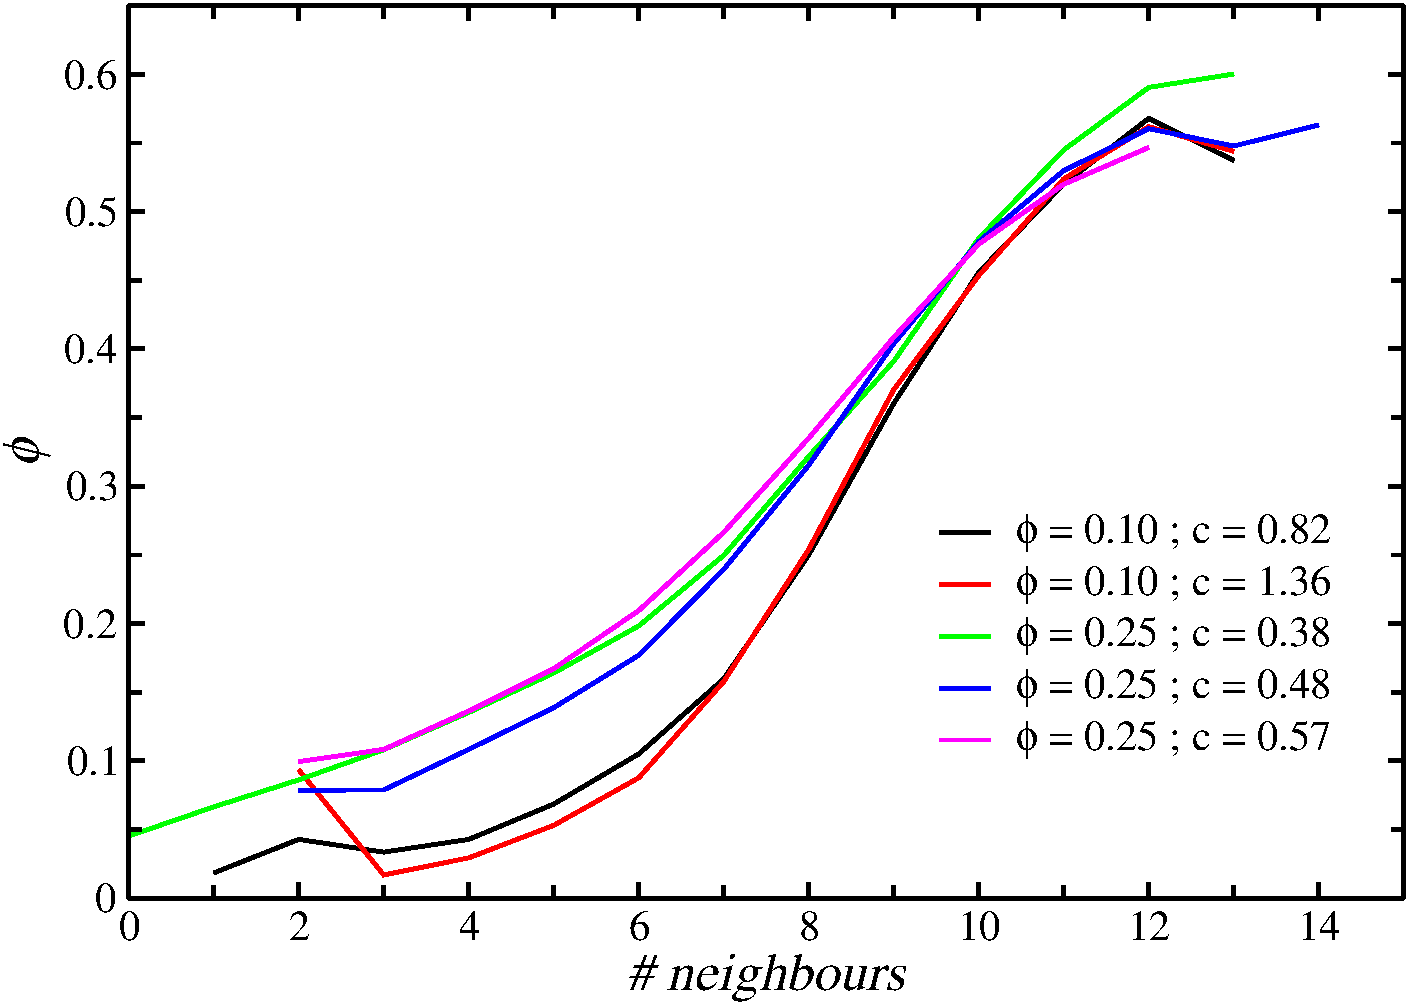
\includegraphics[width=8cm]{oldfig/fig3b}
%  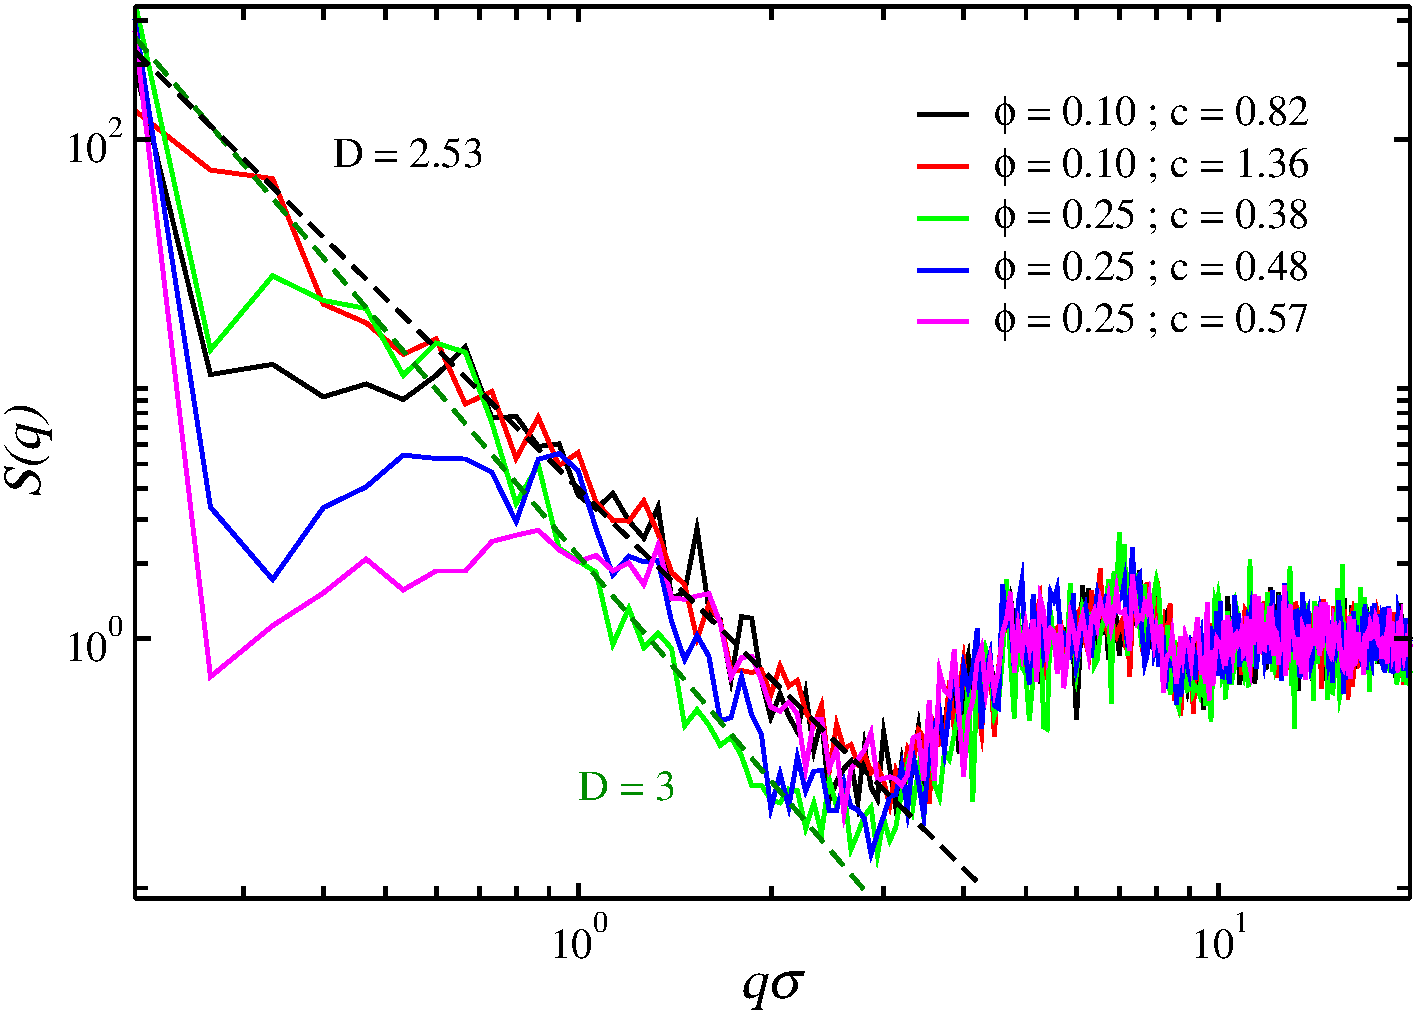
\includegraphics[width=8cm]{oldfig/fig3c}
%  % crystal_size.eps: 0x0 pixel, 300dpi, 0.00x0.00 cm, bb=(atend)
%  \caption{{\bf Two types of arrest mechanism leading to gel formation.} \textbf{a,} Phase diagram \textbf{b,} Local volume fraction around a colloidal particle, as a function of the number of nearest neighbours of the particle.
%  Different lines represent the different state points. {\bf c,} Structure factors for the late stages of the gelation process.} 
%  \label{fig:statepoints}
% \end{figure}


\begin{figure}[!t]
 \centering
 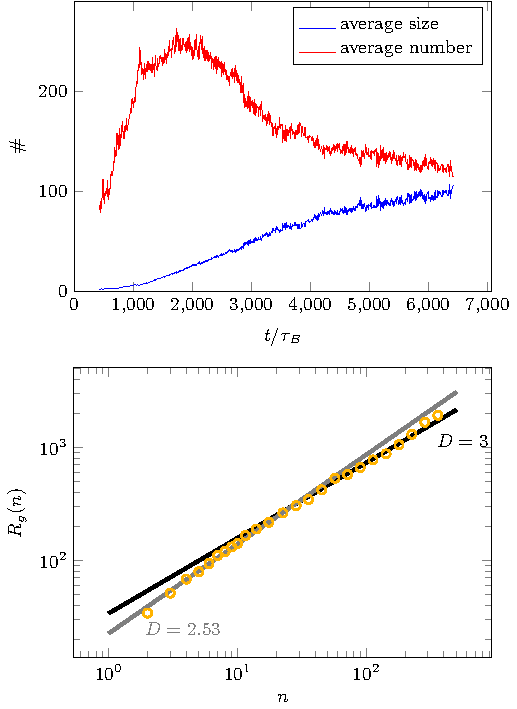
\includegraphics{fig/characterisation.pdf}
 \caption{{\bf Characterisation of the crystal-gel.} {\bf a,} Time evolution of the average size of the crystals (blue line) and the number of crystals (red line) for the state point $\phi=0.25$ and $c_p=0.38$. {\bf d,} Radius of gyration of crystalline nuclei at the late stages of gelation for the same state point.} 
 \label{fig:crystals}
\end{figure}

To confirm the formation of crystalline seeds we adopt bond orientational analysis to detect which particles are in crystalline environments~\cite{russo2012microscopic}. With this analysis we confirm that crystallization events start occurring for the state point $\phi=0.25$ and $c_p=0.38$, which has the lowest
polymer concentration of all state points. This is shown in Fig.~\ref{fig:crystals}a where the black line indicates the average size of the crystallites,
while the red line the average number of crystallites as a function of time. The number of crystallites first rapidly increases as nucleation events
start occurring inside the liquid branches, but eventually starts decreasing as the different crystallites grow and merge with each other.
%The average size of the crystals shows an interesting linear growth regime for $100<t<600$. This linear growth regime goes past the time
%of coalescence of nuclei, so a first speculation is that it could be due to the compensation of the following two effects:
%\begin{itemize}
% \item diffusive growth of the nuclei, which scales like $t^{1/2}$
% \item coalescence growth, which should scale faster than $t$, maybe $t^2?$
%\end{itemize}
All other state points show only negligible signs of crystallization. In particular, for state points with $\phi=0.25$, increasing
polymer concentration drastically reduces the amount of crystals. This is in agreement with the
idea of enhanced crystallization rates near metastable critical points~\cite{ten1997enhancement,olmsted1998spinodal} and the
results of Ref.~\cite{fortini2008crystallization,perez2011pathways},
which speculated two different arrest mechanism: crystallization at low polymer concentration, and dynamic arrest at high polymer concentrations.

While nucleation always occurs inside the liquid branches of the phase separating network, we suggest here the presence of a new growth channel
which was not observed before. In the following we will show that the growth mechanism of the crystal is not only due to filling of the spinodal liquid network, as was observed in Ref.~\cite{fortini2008crystallization,perez2011pathways} for brownian dynamics simulations, but involves direct condensation of the gas phase
on the crystalline seeds.
To investigate this process, we plot in Fig.~\ref{fig:crystals}c the gyration radius of individual crystalline nuclei for the state point
$\phi=0.25$ and $c_p=0.38$. The results show that the crystal growth follows two different scaling laws: at small crystalline sizes it scales with
the dimension of random percolation $D=2.53$, while at large sizes it scales as $D=3$ of compact crystal growth. This demonstrates that, while
small crystalline nuclei are nucleated inside the phase-separated liquid branches, once they reach the transverse size of the liquid branch, the growth
follows a volume expansion with the formation of isotropic droplets (colloidal rain). The same scaling law was suggested in the analysis of the
structure factors, Fig.~\ref{fig:phase_separation}c, but it is shown directly by the analys of the gyration radius.


\begin{figure*}
 \centering
 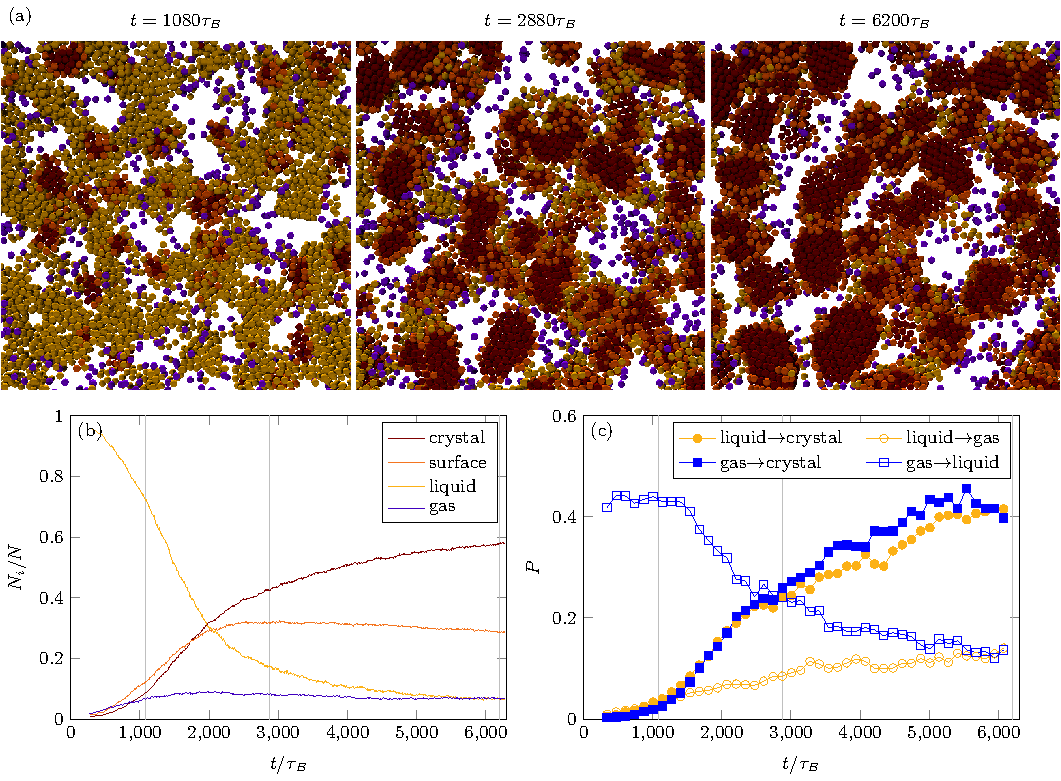
\includegraphics{fig/crystal.pdf}
 \caption{
{\bf Crystal gel formation.} 
\textbf{a,} Reconstructions from confocal coordinates at $\phi=0.25$ and $c_p=0.38$. Depth of view is $5\sigma$. Particles are drawn to scale and coloured according to their phase. Dark red: crystal; orange: surface of crystal; yellow: liquid; blue: gas. 
 \textbf{b,} Fraction of particles for each phase. Gray vertical lines indicate the times shown in \textbf{a.}
\textbf{c,} Transition probabilities for the same process as in \textbf{b}. Here crystal includes surface particles.}
 \label{fig:transitions}
\end{figure*}

In the next section we demonstrate that the volume growth is due to direct condensation of the gas phase on the crystalline seeds.
First we show in Fig.~\ref{fig:transitions}a slabs of 10 particle diameter thickness for configurations at $\phi=0.25$ and $c_p=0.38$ at different times.
Particles are coloured according to their phase. The figure shows the first nucleation
events inside the liquid network (left panel); then these crystalline nuclei grow directly from the gas phase (middle panel), and finally
the different nuclei coalesce (right panel). 

Next we show in Fig.~\ref{fig:transitions}b the fraction of particles in each different phase for the crystallization trajectory at
$\phi=0.25$ and $c_p=0.38$, after the liquid-gas phase separation has occurred. The process of crystallization is characterized
by a steep decrease in liquid particles, as they transform in small crystalline nuclei inside the liquid domains. This decrease
is accompanied by an increase in the fraction of gas particles: as the first crystals start to appear, liquid particles evaporate
to the gas phase due to the highest vapour pressure of the liquid phase compared to the crystalline phase. After the onset
of a steady-state gas population, the crystallization proceeds by adding surface particles to the small crystallites. To confirm this process we
examine in Fig.~\ref{fig:transitions}c the transfer matrix probabilities $P_{\alpha\beta}$, where $\alpha$ and $\beta$ are each of the
phases gas, liquid and crystal (which includes bcc, hcp, fcc and surface particles). Liquid particles undergo two processes, on one
hand they transform to crystallites growing inside the liquid branches of the network, and also increasingly transform to gas particles.
Gas particles first undergo a transition to liquid particles as the final stage of the liquid-gas phase separation, but once
crystalline nuclei outgrow the liquid pockets in which they are formed, the probability for the transition from gas to liquid
abruptly decreases. Instead, gas particles start depositing on the crystal, and at later stages the pace of the gas-to-crystal transformation
is larger than the one of the liquid-to-crystal one.

We can thus conclude that the crystallization proceeds via two distinct mechanisms:
(i) freezing of the fluid; (ii) evaporation of the fluid and condensation of the vapor on the crystals.
The first process dominates the initial stages of crystallization, while the second one becomes effective once
crystalline nuclei have outgrown the liquid regions in which they form. 
% 
% Here we mention the simulations closer to our experimental results~\cite{fortini2008crystallization}.
% It was shown there that close to the metastable liquid-gas critical point, the gelation process is arrested by
% crystallization, while at higher polymer concentration by slow dynamics. This is roughly what we observe in
% our experiments, but there is a crucial difference. In the simulation results~\cite{fortini2008crystallization} the kinetic
% pathway at volume fraction $\phi=0.25$ consists of the following three steps: 
% spinodal decomposition; nucleation of crystalline nuclei within the fluid branches;
% growth of crystalline clusters until the whole spinodal structure is crystalline.
% As shown above, the last step appears to be markedly different in our experiments.
% More precisely, at $\phi=0.25$ and polymer concentration $c_p=0.38$ we also observe the first two steps, 
% but the growth process is entirely different. Instead of growing inside
% the spinodal aggregate, the small nuclei grow by adding colloids directly from the gas phase. 

\subsection*{Discussion and conclusions}
The first stages of gelation always involve spinodal decomposition with the formation
of a fractal network and gas-liquid phase separation.
% Due to hydrodynamic interaction, the network is locally stretched, and the accumulation of mechanical stress on some bonds causes some
% of them to break and the network to reorganize in a more compact and larger structure. This occurs only at low polymer concentration,
% while at high polymer concentrations the bonds are too strong to break. This will eventually dictate which arrest mechanism
% is available to the system.
Depending on the polymer concentration, there are two possible arrest mechanisms.
(i) Crystallization, observed at $\phi=0.25$ and $c_p=0.38$, small crystalline nuclei appear inside the liquid, reach the surface
 of the liquid branches, and then grow by addition of particles from the gas phase. The final structure is a network of crystal droplets,
 as confirmed by the fractal dimension of the branches, the volume fraction of the particles within the branches, and bond orientational analysis.
(ii) Dynamic arrest, particle arrest when the dynamics inside the liquid branch becomes slow, which should happen at the intersection of the
 glass line with the liquid side of the coexistence curve.

The process we observed is akin to the Bergeron process which is the primary mechanism for the formation of raindrops in clouds~\cite{glickman2000glossary}.
In clouds there is a mixture of ice crystals and supercooled water. The vapor phase is in coexistence with the liquid phase, but is supersaturated
with respect to the ice crystals. This causes the water droplets to evaporate and sublimate directly on the ice crystals. Our system can then
be regarded as a colloidal analogue for this important process, which can now be studied at the single-particle level.
The basic mechanism creating ``crystal gels'' may be generic to many other
systems. The requirements are (i) the presence of gas-liquid phase separation below the melting point of a crystal, (ii) 
weak or little frustration against crystallization (in our case, the use of monodisperse colloids), 
(ii) dynamical slowing down in a supercooled liquid state, which is necessary to induce viscoelastic phase separation leading to the formation 
of a network structure of the minority phase, and (iii) the degree of supercooling is low enough to avoid a high rate of densification of the liquid phase 
leading to vitrification.   
Many monoatomic and single-component molecular systems can satisfy all these conditions in a certain range of the temperature and pressure. 
This can be seen, for example, by looking at the phase diagram of a Lennard-Jones liquid, which represents many molecular systems 
without specific directional interactions. So we believe that crystal gels are an important class of heterogeneous non-ergodic states in nature 
and industrial applications, although they have not attracted much attention so far.  

\section*{Methods}

\paragraph*{Experimental}
We use \textsc{pmma} (poly(methyl methacrylate)) colloids sterically stabilized with methacryloxypropyl terminated \textsc{pdms}(poly(dimethyl siloxane)) and fluorescently labelled with rhodamine isothiocyanate chemically bonded to the \textsc{pmma}. We disperse the particles in refractive index and density matching mixture of cis-decalin (Tokyo Kasei) and bromocyclohexane (Sigma-Aldrich).

To induce short-ranged depletion attraction, we use polystyrene (TOSOH) of molecular weight \SI{3.8}{\mega\dalton} as non-adsorbing polymer. Experiments are conducted at \SI{27}{\celsius}, some \SI{80}{\celsius} above the theta temperature in this solvents mixture~\cite{Royall2007}. A Flory scaling of the measurements of~\cite{lu2008gelation} yields a radius of gyration $R_g=\SI{76}{\nano\metre}$.

In the absence of salt, the Debye length is expected to reach several \si{\micro\metre} and the (weakly) charged colloids experience a long range electrostatic repulsion. We confirm that colloids never come close enough to feel the short-ranged attraction. Screening by tetrabutylammonium bromide (Fluka) at saturated concentration brings down the Debye length to about \SI{100}{\nano\metre}, practically discarding the repulsion.

The data are collected on a Leica SP5 confocal microscope, using \SI{532}{\nano\metre} laser excitation. We assess that the size distribution of our particle is Gaussian with a polydispersity below 5\% via direct confocal measurements~\cite{Leocmach2013}. The mean diameter is $\sigma=\SI{2.1}{\micro\metre}$ XXX to be checked XXX yielding a size ratio $q_R=2R_g/\sigma=0.07$. The Brownian time is $\tau_B \approx \SI{4.5}{\second}$. To be able to follow individual trajectories, we perform a 3D scan every \SI{10}{\second} at early time and every \SI{30}{\second} later.

%\paragraph*{State points studied}
%The experimental data is taken at two different volume fractions ($\phi=0.10$ and $\phi=0.25$) and for different values
%of the polymer concentration, $c_p=0.38,0.48,0.57,1.07$ for $\phi=0.25$ and $c_p=0.82,1.36$ for $\phi=0.10$.
%For each state points, scans at early times (every $10s$) and at the late stage (every $30s$) of the gelation process.
%
%We will consider two particles bonded if their center-to-center distance is within $12$ pixels. The radius of a colloidal
%particle is $5.365$ pixels.

\paragraph*{Structural analysis}
To account for imprecision in particle localisation close to contact, we consider two particles bonded if their center-to-center distance is within $\SI{2.3}{\micro\metre}>\sigma+2R_g$.

To detect percolation, two different methods have been employed. In the first one we detect percolation
by looking at which frame the cluster size distribution has a more extended power-law decay. In the second technique,
we simply measure the spatial extent of the largest cluster and consider it percolating when it is comparable to the
size of the field of view of the microscope. Both methods lead to essentially identical percolation time for each state point.

Crystalline phases are detected through bond orientational analysis~\cite{russo2012microscopic}, they are mainly FCC and HCP in comparable proportions. Surface particles are particles with at least two crystalline neighbours; liquid particles have at least 4 neighbours; gas particles are particles with less than 4 nearest neighbours.

\bibliographystyle{naturemag4}
\bibliography{biblio}

\clearpage










\end{document}



\section{Future things to do}
Is the absence of network restructuring that is preventing crystallization?